\section{Исследовательская часть}

\subsection{Результаты работы разработанного ПО}

На рисунке \ref{fig:modinfo} представлена информация о разработанном загружаемом модуле ядра и его логи. На рисунке \ref{fig:example} -- пример работы модуля, а на рисунке \ref{fig:free-m} -- сравнение результатов его работы с результатами команды <<free -m>> (у последней все объемы указаны в Мб).

\begin{figure}[h!]
	\begin{center}
		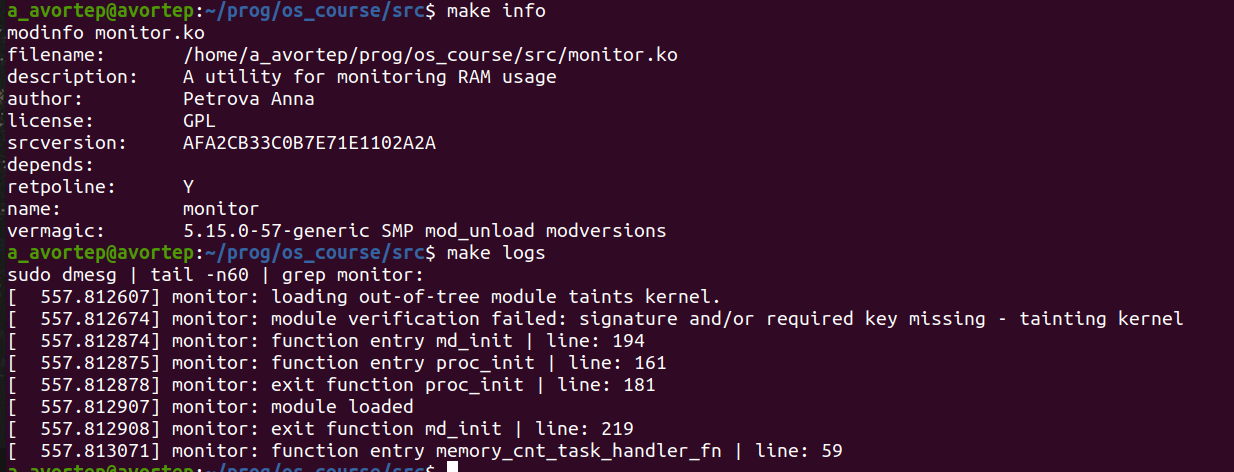
\includegraphics[scale=0.38]{jpg/1.png}
	\end{center}
	\captionsetup{justification=centering}
	\caption{Информация о модуле и логи}
	\label{fig:modinfo}
\end{figure}

\begin{figure}[h!]
	\begin{center}
		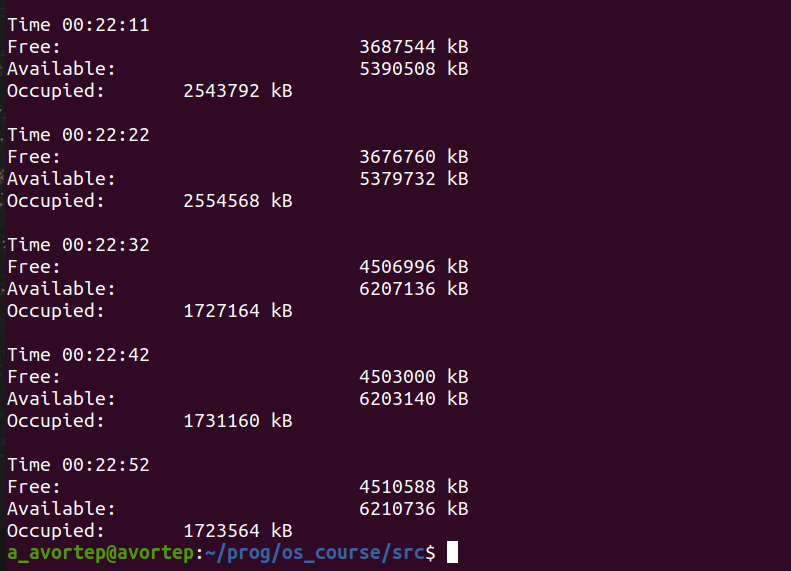
\includegraphics[scale=0.4]{jpg/2.png}
	\end{center}
	\captionsetup{justification=centering}
	\caption{Пример работы модуля}
	\label{fig:example}
\end{figure}

\begin{figure}[h!]
	\begin{center}
		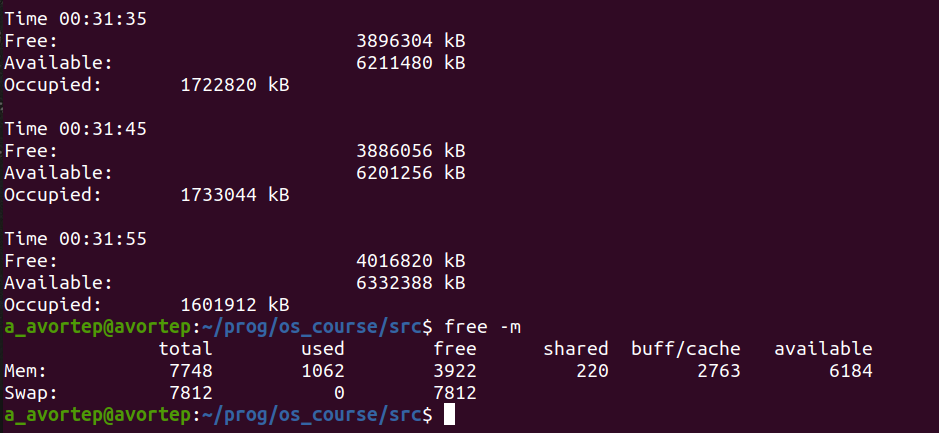
\includegraphics[scale=0.45]{jpg/3.png}
	\end{center}
	\captionsetup{justification=centering}
	\caption{Результаты работы команды <<free -m>>}
	\label{fig:free-m}
\end{figure}

На рисунке \ref{fig:graphic} представлена визуализация данных о свободной, доступной и занятой памяти в системе, полученных из разработанного модуля ядра.

\begin{figure}[h!]
	\begin{center}
		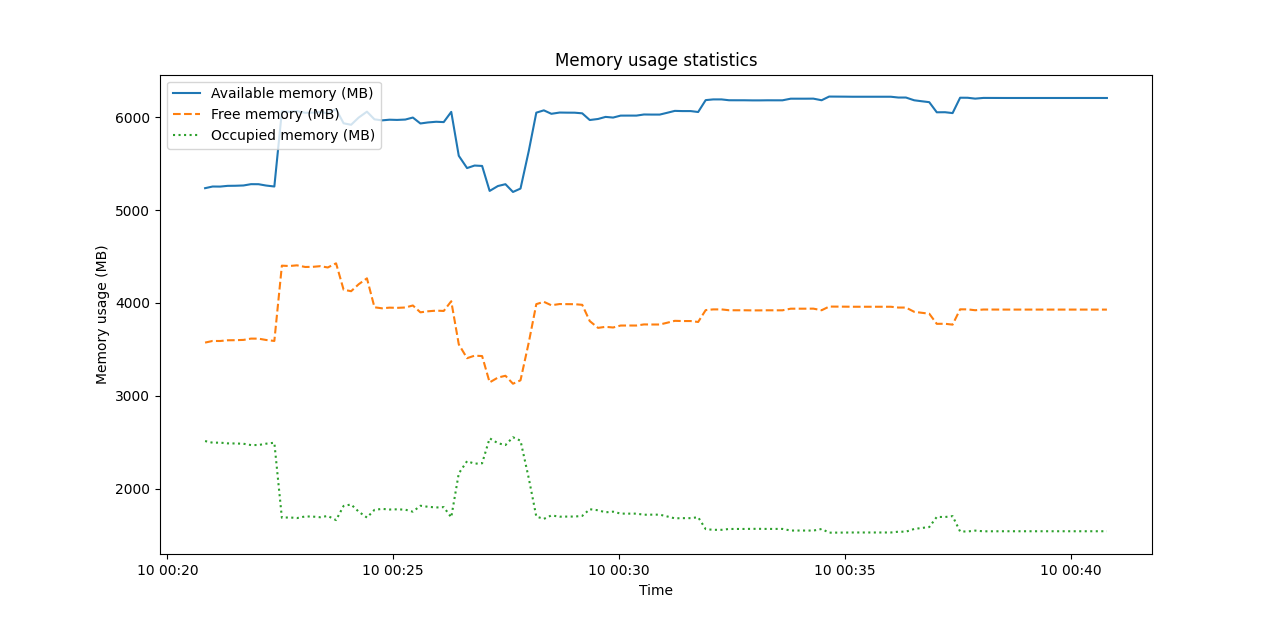
\includegraphics[scale=0.55]{jpg/memory_usage.png}
	\end{center}
	\captionsetup{justification=centering}
	\caption{Визуализация данных о памяти за 20 минут}
	\label{fig:graphic}
\end{figure}

\newpage

\subsection{Анализ результатов}

На основе рисунка \ref{fig:free-m} можно сделать вывод, что результаты работы разработанного загружаемого модуля ядра совпадают с результатами работы команды <<free -m>>. Следовательно, результаты корректны.

По рисунку \ref{fig:graphic} видно, как изменялась загруженность памяти в течение 20 минут. В моменты резкого спада количества занятой оперативной памяти было закрыто несколько приложений, а в моменты роста -- наоборот, открыто.

\subsection*{Выводы}
В данном разделе были приведены результаты работы разработанного ПО и проведён анализ этих результатов. 

В итоге было выяснено, что результаты работы модуля корректны, так как совпадают с результатами работы стандартной команды. Также по приведенному выше графику была выявлена зависимость загруженности оперативной памяти от количества запущенных приложений.

